\documentclass{beamer}
\usepackage[utf8]{inputenc}

\usepackage{listings}
\usepackage{color}
\usepackage{verbatim}

%New colors defined below
\definecolor{codegreen}{rgb}{0,0.6,0}
\definecolor{codegray}{rgb}{0.5,0.5,0.5}
\definecolor{codepurple}{rgb}{0.58,0,0.82}
\definecolor{backcolour}{rgb}{0.95,0.95,0.95}

%Code listing style named "mystyle"
\lstdefinestyle{mystyle}{
  backgroundcolor=\color{backcolour},   
  commentstyle=\color{codegreen},
  keywordstyle=\color{blue},
  numberstyle=\tiny\color{codegray},
  stringstyle=\color{codepurple},
  basicstyle=\footnotesize,
  breakatwhitespace=false,         
  breaklines=true,                 
  captionpos=b,                    
  keepspaces=true,                 
  numbers=left,                    
  numbersep=5pt,                  
  showspaces=false,                
  showstringspaces=false,
  showtabs=false,                  
  tabsize=2
}

%"mystyle" code listing set
\lstset{style=mystyle}

\title{Seeding Strategies for Lloyd`s kmeans}
\subtitle{C++ implementation of Ostrovsky, Rabani, Schulman and Swamy`s ideas}
\author{Mirko Speth}
\date{22.07.2016}
\subject{Computer Science}

\begin{document}

  \frame{\titlepage}
  \begin{frame}
    \frametitle{Overview}
    Five approaches to seed Lloyd`s k-means
    \begin{itemize}
        \item{A: Random Sampling}
        \item{B: Greedy Deletion}
        \item{C: Linear time algorithm}
        \item{D: Linear time constant factor algorithm}
        \item{E: Polynomial Time Approximation Scheme (PTAS)}
    \end{itemize}
  \end{frame}
  
  
  
  
  \begin{frame}
    \frametitle{A: Random Sampling}
    \framesubtitle{$O(knd)$}
    \begin{enumerate}
        \item Select two random points $c_1$ and $c_2$ with probability $||c_1-c_2||^2$
        \item Perform a ball-k-means step
        \item Repeat: add another point $c_{i+1}$ with probability $min_{j\in\{1...i\}}{||c_{i+1}-c_j||^2}$
    \end{enumerate}
  \end{frame}
  
  \begin{frame}[fragile]
\frametitle{A: Random Sampling}
\begin{figure}[ht]
	\centering
	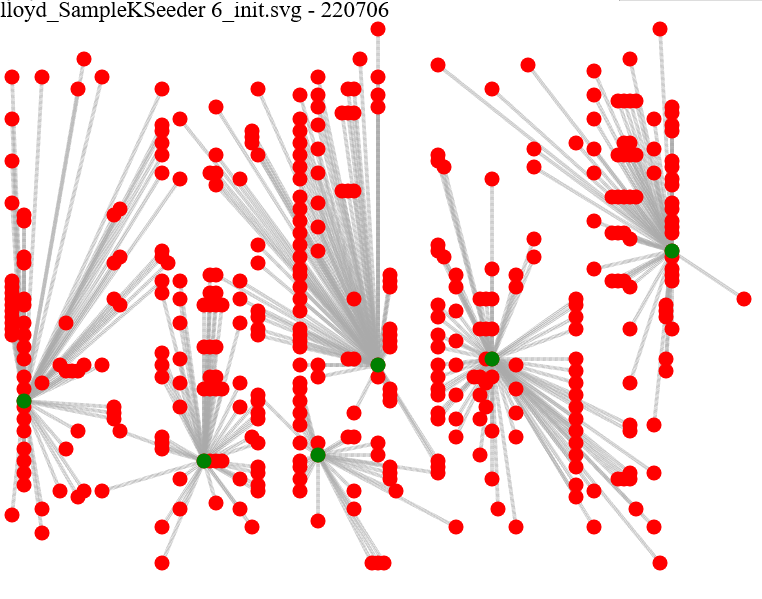
\includegraphics[scale=0.4]{SamplekSeeder_pbl395.PNG}
	\caption{SVG-Output of SamplekSeeder on pbl395.tsp (k=6)}
\end{figure}
\end{frame}
  
  \begin{frame}[fragile]
    \frametitle{B: Greedy Deletion}
\begin{lstlisting}[language=C++]
Pointset GreedyDelSeeder::seed(Pointset init) const {
	Pointset sites = init;
	while (sites.size() > (unsigned int) k) {

		// B1: get best and second best center for each customer
		Partition part = Partition(&customers, sites);

		// B2: pick the center for which Tx is minimum
		int bestid = part.getMinTx();

		// B3: delete chosen partition and move points to centroid of voronoi region
		part.delete_set_from_partition(bestid);
		sites = part.centroids();
	}
	return sites;
}
\end{lstlisting}
\end{frame}



  \begin{frame}
    \frametitle{B: Greedy Deletion}
    Running time: outer loop $(n-k)$ iterations $\Rightarrow O(n)$\\
    Partitioning: $O(n^2d)$\\
    No speed loss for second best\\
    $\Rightarrow$ together: $O(n^3d)$
  \end{frame}

  
    \begin{frame}[fragile]

    \frametitle{C: Linear time algorithm}
\begin{lstlisting}[language=C++]
Pointset LTSeeder::seed() const {

	//C1
	double e = instance.eps();
	double p1 = sqrt(e);
	int N = (int)(2 * k / (1 - 5 * p1) + 2 * log(2 / p1) / pow((1 - 5 * p1), 2));

	SampleKSeeder samplekseeder(instance, N);
	Pointset S = samplekseeder.seed();

	//C2
	Partition partition = Partition(&customers, S);
	Pointset sdach = partition.centroids();

	GreedyDelSeeder greedydelseeder(instance, k);

	return greedydelseeder.seed(sdach);
}
\end{lstlisting}
\end{frame}

\begin{frame}[fragile]
\frametitle{C: Linear time algorithm}
$O(nkd +k^3d)$
\begin{figure}[ht]
	\centering
	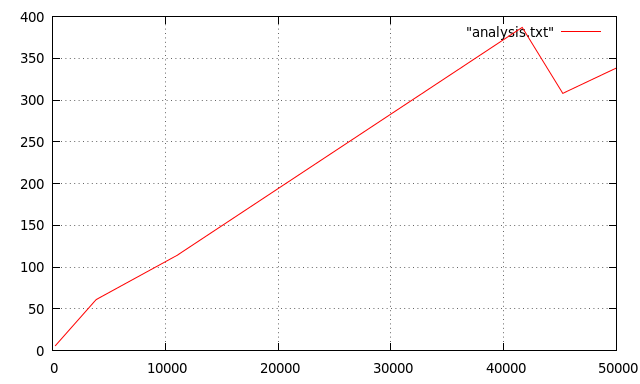
\includegraphics[scale=0.2]{LTSeeder_complexity_in_n.png}
	\caption{complexity in \#customers}
\end{figure}
\begin{figure}[ht]
	\centering
	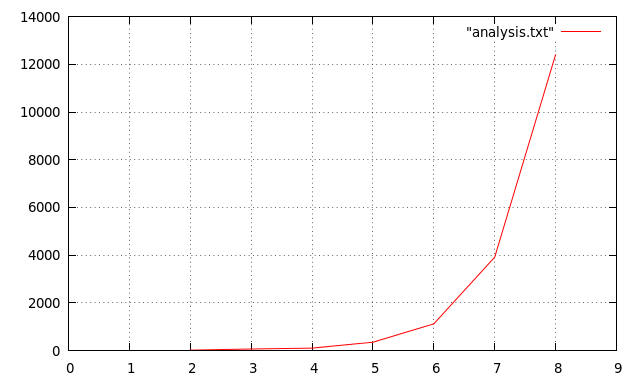
\includegraphics[scale=0.2]{LTSeeder_complexity_in_k.png}
	\caption{complexity in \#sites}
\end{figure}
\end{frame}

  
      \begin{frame}[fragile]

    \frametitle{D: Linear time constant factor algorithm}
\begin{lstlisting}[language=C++]
Pointset DSeeder::seed() const {
    // D1 (obtain k initial centres using last seeding strategy)
	Pointset init = (LTSeeder(instance, k)).seed();

	// D2 (run a ball-k-means step)
	return ballkmeansstep(init);
}
\end{lstlisting}
\end{frame}

\begin{frame}[fragile]
\frametitle{D: Linear time algorithm}
\begin{figure}[ht]
	\centering
	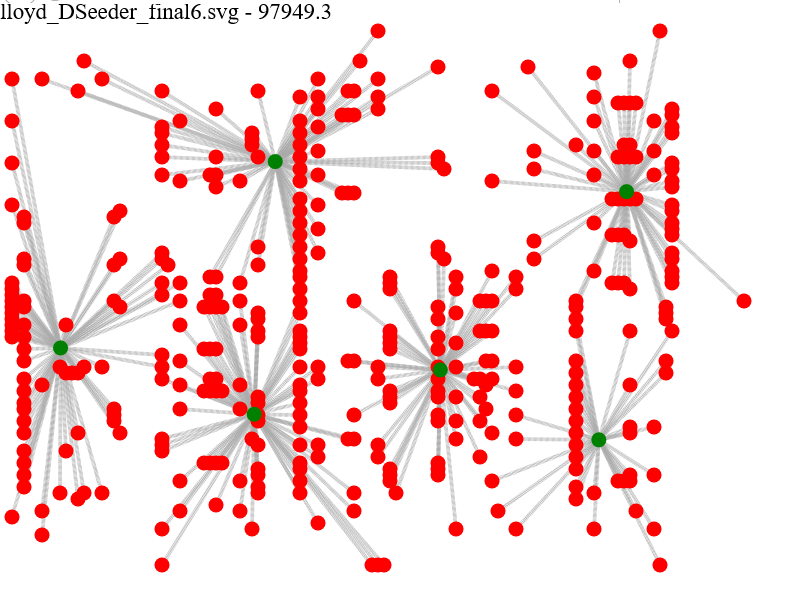
\includegraphics[scale=0.4]{DSeeder_pbl395.PNG}
	\caption{SVG-Output of DSeeder on pbl395.tsp (k=6)}
\end{figure}
\end{frame}

  
\begin{frame}[fragile]
    \frametitle{E: Polynomial Time Approximation Scheme (PTAS)}
\begin{lstlisting}[language=C++]
Pointset ESeeder::seed() const {
	SampleKSeeder samplek(instance, k);
	Partition part = Partition(&customers, samplek.seed());
	return part.centroid_estimation(instance.omega, instance.eps);
}
\end{lstlisting}
\end{frame}


\begin{frame}[fragile]
\frametitle{centroid estimation}
\begin{lstlisting}[language=C++]
for s in sites:
    select expanded Voronoi region V[s]
    choose a random subset R[s] of V[s] of size 4/wb
    foreach subset A of size 1/wb:
        add centroid(A) to T[s]
foreach set B in {{x1,...xk} : xi in T[i]}:
    if error(B) < error (best) then best = B
\end{lstlisting}
\end{frame}

\begin{frame}[fragile]
\frametitle{PTAS analysis}
Ostrovski et al:\\ 
error at most $(1+\omega)*OPT$ with probability $\gamma^k$\\ 
(for some constant $\gamma$)
\end{frame}

\begin{frame}[fragile]
\frametitle{E: PTAS}
$O(2^{(\frac{4k}{\beta\omega})}n*d)$
\begin{figure}[ht]
	\centering
	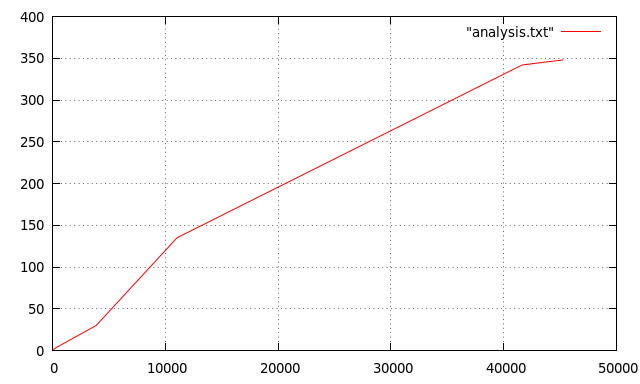
\includegraphics[scale=0.2]{ESeeder_complexity_in_n.png}
	\caption{complexity in \#customers}
\end{figure}
\begin{figure}[ht]
	\centering
	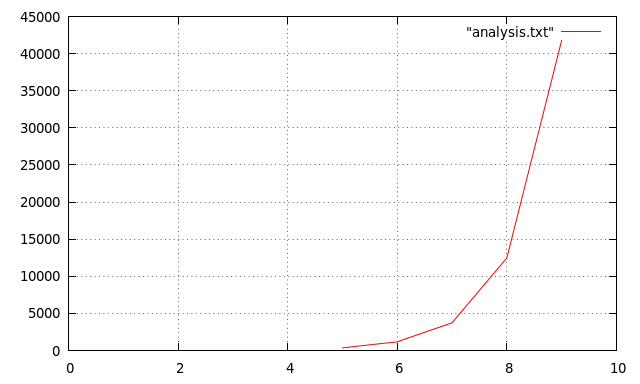
\includegraphics[scale=0.2]{ESeeder_complexity_in_k.png}
	\caption{complexity in \#sites}
\end{figure}
\end{frame}

\begin{frame}[fragile]
\frametitle{Comparison}
\begin{figure}[ht]
	\centering
	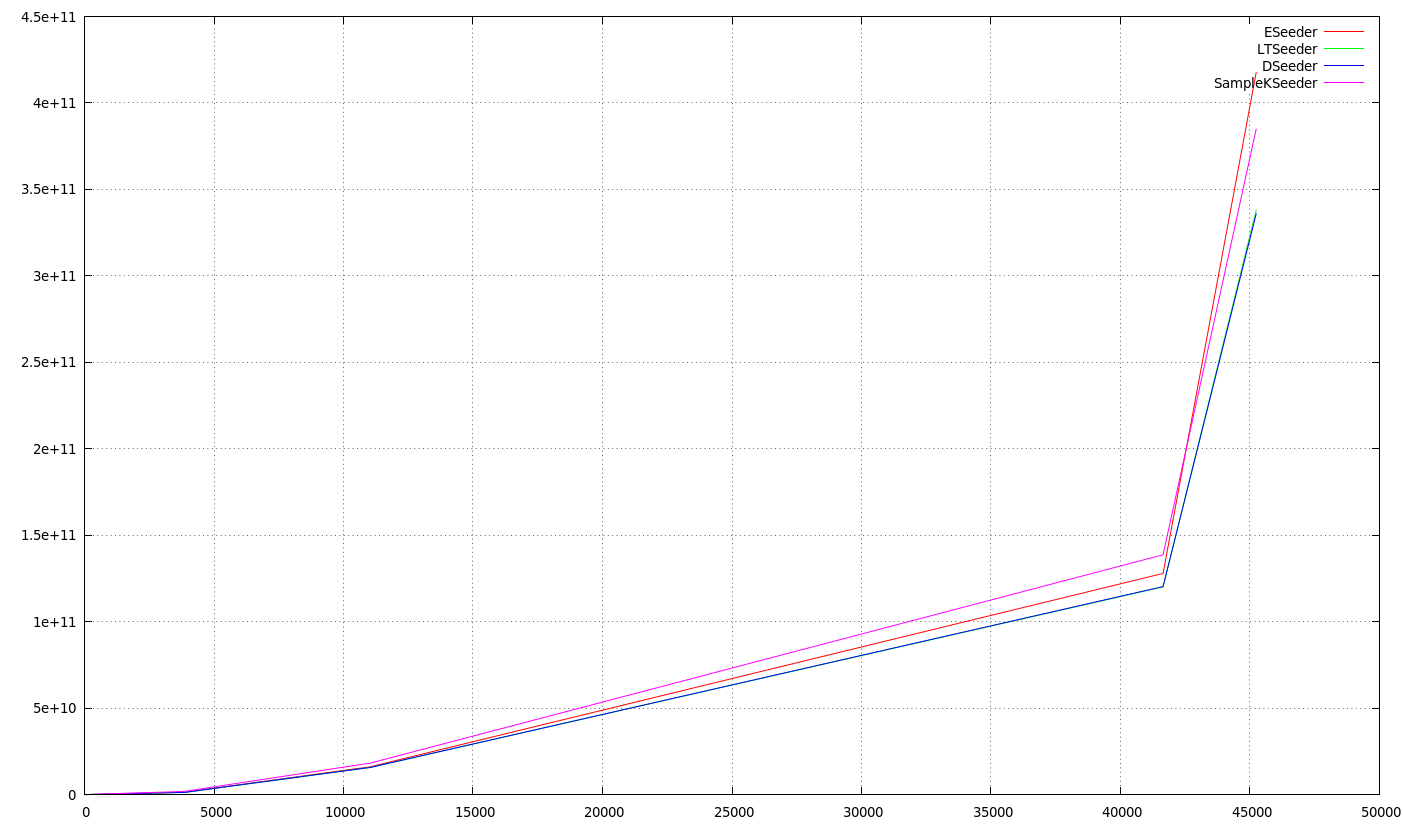
\includegraphics[scale=0.1]{resultcompare.png}
	\caption{error comparison}
\end{figure}
\begin{figure}[ht]
	\centering
	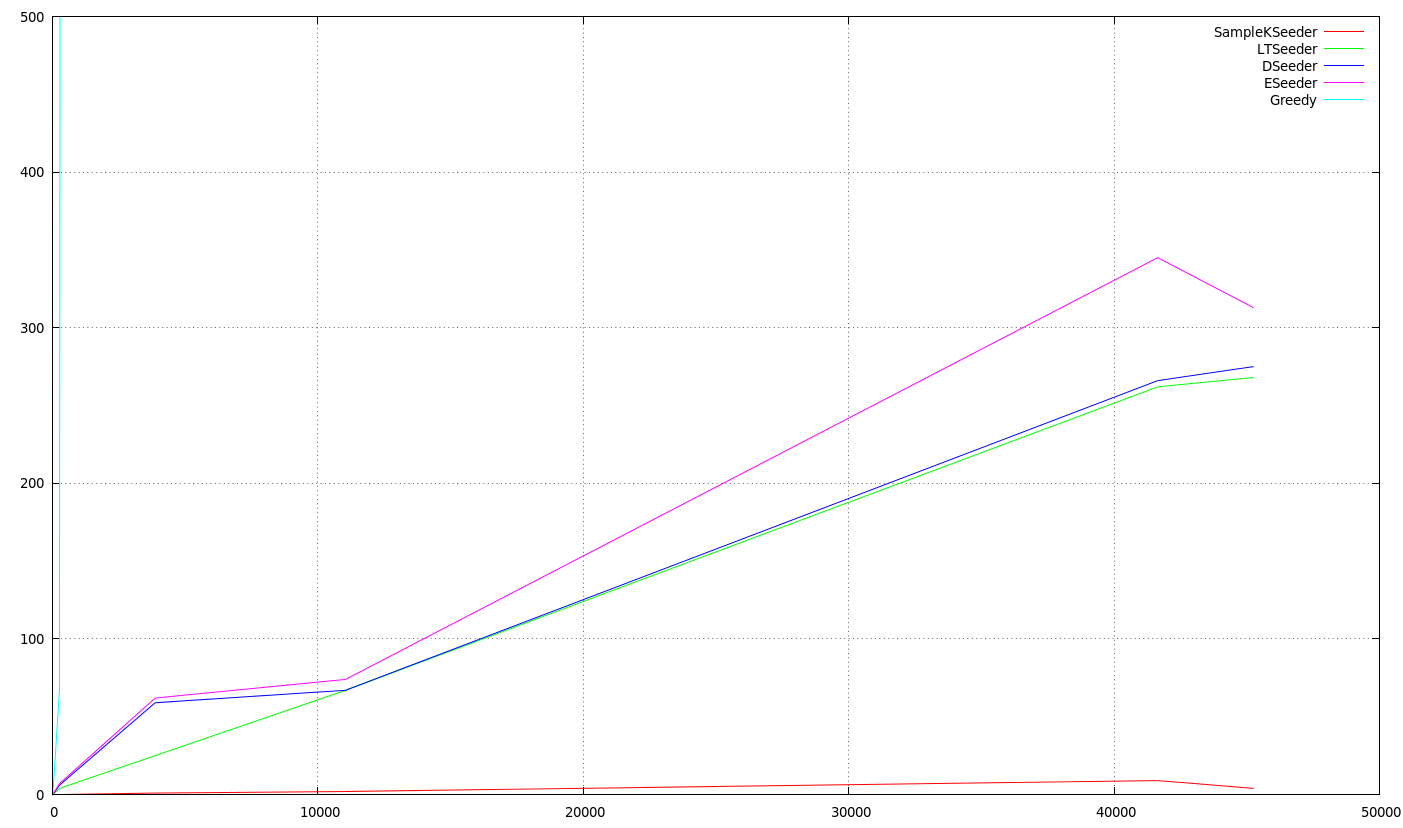
\includegraphics[scale=0.1]{runtimecompare.png}
	\caption{runtime comparison}
\end{figure}
\end{frame}


  

\end{document}
